%
% einleitung.tex -- Beispiel-File für die Einleitung
%
% (c) 2020 Prof Dr Andreas Müller, Hochschule Rapperswil
%
% !TEX root = ../../buch.tex
% !TEX encoding = UTF-8
%

\section{Grundlagen der Fourier-Analyse\label{fourier:section:teil0}}
\kopfrechts{Teil 0}

Die Fourier-Analyse ist ein sehr mächtiges Mittel in der Signal-Analyse. 
Einleitung...


\subsection{Fourierreihe\label{fourier:subsection:fourierreihe}}

Mit der Fourier-Reihe lassen sich periodisch wiederholende Funktionen, wie ein Rechteck- oder Dreiecksignal, mit skalierten Sinus- und Kosinus-Schwingungen darstellen.
Um die Reihe aufzustellen, braucht man nur 3 Koeffizienten zu bestimmen. 

\begin{itemize}
	\item $a_0$ ist der Mittelwert, der Funktion. 
	Dieser entspricht dem Integral über eine Periode und schliesslich geteilt durch die Periode. 
	
	\begin{equation}
		a_0 = \frac{1}{T} \int_{t_0}^{t_0 + T} f(t) \, dx
	\end{equation}
	
	\item $a_n$ beschreibt den geraden Anteil der Funktion.
	
	\begin{equation}
		a_n = \frac{2}{T} \int_{t_0}^{t_0 + T} f(t) \cos\left(\frac{2\pi n t}{T}\right) dt
	\end{equation}
	
	\item $b_n$ beschreibt den ungeraden Anteil der Funktion.
	
	\begin{equation}
		b_n = \frac{2}{T} \int_{t_0}^{t_0 + T} f(t) \sin\left(\frac{2\pi n t}{T}\right) dt
	\end{equation}
	
\end{itemize}

Mit allen Koeffizienten bestimmt lässt sich die ursprüngliche Funktion nachamen. 

Mit der Grafik ??? lässt sich dies schön zeigen.

\[
f(t) = \frac{a_0}{2} + \sum_{n=1}^{\infty} \left( a_n \cos\left( \frac{2\pi n}{T} x \right) + b_n \sin\left( \frac{2\pi n}{T} x \right) \right)
\]

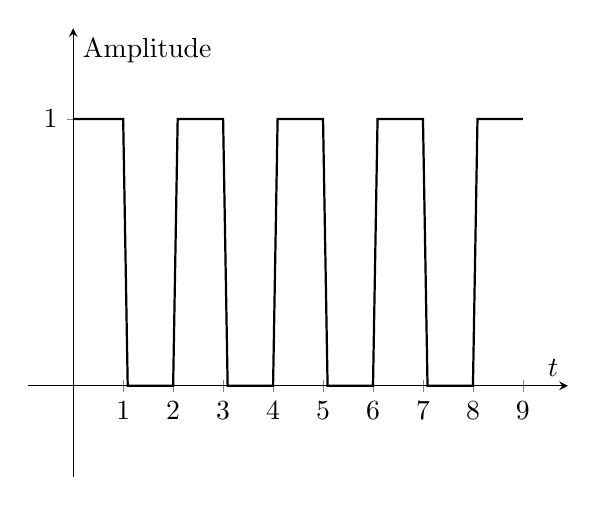
\begin{tikzpicture}
	\begin{axis}[
		axis lines = middle,
		xlabel = {$t$},
		ylabel = {Amplitude},
		domain=0:9,
		samples=100,
		xtick={0,1,2,3,4,5,6,7,8,9},
		ytick={0,1},
		ymin=-0.2, ymax=1.2, 
		enlargelimits
		]
		\addplot[thick] {mod(floor(x),2) == 0 ? 1 : 0};
	\end{axis}
\end{tikzpicture}

De abschnitt isch nur mal grob gmacht, wird scho no überarbeitet.
Ich plan no die fourier Reihe über die funktion z lege. maybe no s gibbsche phenomen a spreche. 


\subsection{Fouriertransformation\label{fourier:subsection:fouriertransformation}}

